

\section{Tabular Data Structure}
This package also provides support for a tabular datatype.
The string representation of the table datatype is a matrix, with the first row being the header.
The values in the first column must be unique, and are called the table's ``keys''. 
Correspondingly, the first header entry is called the ``keyname'', and the remaining header entries are the table's ``fields''. 
The rest of the matrix is the table's data, accessible by indexing with keys and fields.
Missing values are represented by blanks.
The conceptual layout of the table is illustrated in the figure below.
\vspace{\baselineskip}
\FloatBarrier
\begin{figure}[!htb]
    \centering
    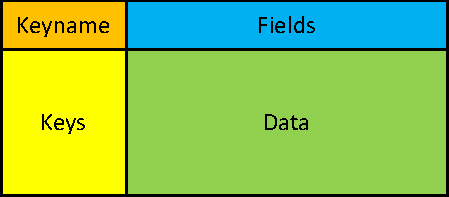
\includegraphics{figures/table.pdf}
    \caption{Conceptual Representation of Tabular Data Structure}
    \label{fig:table_props}
\end{figure}

The command \cmdlink{table} is a TclOO class based on the superclass \textit{::vutil::ValueContainer}, from the package \textcolor{blue}{\href{https://github.com/ambaker1/vutil}{vutil}}. 
It is an object-oriented approach to tabular data manipulation.
\begin{syntax}
\command{table} new \$varName <\$value>
\end{syntax}
\begin{syntax}
table create \$name \$varName <\$value>
\end{syntax}
\begin{args}
\$varName & Variable to store object name for access and garbage collection.  \\
\$value & Matrix representation of table. Default blank. \\
\$name & Name of object if using ``create'' method.
\end{args}

\begin{example}{Creating and accessing a table}
\begin{lstlisting}
table new tableObj {{key A B} {1 foo bar} {2 hello world}}
puts [$tableObj]
\end{lstlisting}
\tcblower
\begin{lstlisting}
{key A B} {1 foo bar} {2 hello world}
\end{lstlisting}
\end{example}


\clearpage

\subsection{Basic Operators}
Because the table class is a subclass of \textit{::vutil::ValueContainer}, it has the same operator methods. 

The copy operator, ``\texttt{-{}->}'', copies the table to a new variable, and returns the new object.
\begin{syntax}
\index{table methods!-{}->} \$tableObj -{}-> \$varName
\end{syntax} 
\begin{args}
\$varName & Variable to store object name for access and garbage collection. 
\end{args}

The assignment operator, ``\texttt{=}'', sets the value of the entire table, and the math assignment operator, ``\texttt{:=}'', sets the value after passing the input through the \cmdlink{expr} command. 
Both operators return the object.

\begin{syntax}
\index{table methods!-{}->} \$tableObj = \$value
\end{syntax}
\begin{syntax}
\index{table methods!-{}->} \$tableObj := \$expr
\end{syntax}

\begin{args}
\$value & Value to assign. \\
\$expr & Expression to evaluate.
\end{args}

The pipe operator, ``\texttt{|}'', copies the table to a temporary object, and evaluates the method.
Returns the result of the method, or the value of the temporary object.
This operator is useful for converting methods that modify the object to methods that return a modified value.

\begin{syntax}
\index{table methods!$\vert$} \$tableObj | \$method \$arg ...
\end{syntax}

\begin{args}
\$method & Method to evaluate. \\
\$arg ... & Arguments to pass to method.
\end{args}

The ampersand operator ``\texttt{\&}'' copies the table value to a reference variable, and evaluates a body of script. 
The changes made to the reference variable will be applied to the object, and if the variable is unset, the object will be deleted.
If the variable is unset in the script, the object will be destroyed.
Returns the result of the script.

\begin{syntax}
\index{table methods!\&} \$tableObj \& \$refName \$body
\end{syntax}
\begin{args}
\$refName & Variable name to use for reference. \\
\$body & Body to evaluate.
\end{args}

\clearpage

%\begin{example}{Example table}
%\begin{lstlisting}
%table new t {
%    {key x y z}
%    {1 3.44 7.11 8.67}
%    {2 4.61 1.81 7.63}
%    {3 8.25 7.56 3.84}
%    {4 5.20 6.78 1.11}
%    {5 3.26 9.92 4.56}
%}
%puts [$tblObj]
%\end{lstlisting}
%\tcblower
%\begin{lstlisting}
%{key x y z} {1 3.44 7.11 8.67} {2 4.61 1.81 7.63} {3 8.25 7.56 3.84} {4 5.20 6.78 1.11} {5 3.26 9.92 4.56}
%\end{lstlisting}
%\end{example}

\subsection{Wiping, Clearing, and Cleaning a Table}
The method \methodlink[0]{table}{wipe} removes all data from a table object, so that its state is the same as a fresh table.
The method \methodlink[0]{table}{clear} only removes the data and keys stored in the table, keeping the fields and other metadata.
The method \methodlink[0]{table}{clean} only removes keys and fields that have no data.
\begin{syntax}
\method{table}{wipe}
\end{syntax}
\begin{syntax}
\method{table}{clear}
\end{syntax}
\begin{syntax}
\method{table}{clean}
\end{syntax}

\begin{example}{Cleaning the table}
\begin{lstlisting}
table new tableObj
$tableObj = {
    {key x y z}
    {1 {} foo bar}
    {2 {} hello world}
    {3 {} {} {}}
}
puts [$tableObj]
# Remove keys and fields with no data
$tableObj clean
puts [$tableObj]
# Remove all keys and data, keep fields
$tableObj clear
puts [$tableObj]
# Reset table 
$tableObj wipe
puts [$tableObj]
\end{lstlisting}
\tcblower
\begin{lstlisting}
{key x y z} {1 {} foo bar} {2 {} hello world} {3 {} {} {}}
{key y z} {1 foo bar} {2 hello world}
{key y z}
key
\end{lstlisting}
\end{example}
\clearpage

\subsection{Table Access}
The matrix representation of the table can be accessed by calling the object without any methods. 
In addition, the four parts of the table can be accessed with the methods \methodlink[0]{table}{keyname}, \methodlink[0]{table}{keys}, \methodlink[0]{table}{fields}, and \methodlink[0]{table}{values}.

The keyname of a table can be accessed or modified directly with their respective methods. 
\begin{syntax}
\method{table}{keyname}
\end{syntax}
\begin{syntax}
\method{table}{keys} <\$pattern>
\end{syntax}
\begin{syntax}
\method{table}{fields} <\$pattern>
\end{syntax}
\begin{syntax}
\method{table}{values} <\$filler>
\end{syntax}
\begin{args}
\$pattern & Glob pattern to filter keys/fields with. Default ``\texttt{*}'' for all. \\
\$filler & Filler for missing values, default blank.
\end{args}

\begin{example}{Access table components}
\begin{lstlisting}
table new tableObj
$tableObj = {
    {key A B}
    {1 foo bar}
    {2 hello world}
}
puts [$tableObj]
puts [$tableObj keyname]
puts [$tableObj keys]
puts [$tableObj fields]
puts [$tableObj values]
\end{lstlisting}
\tcblower
\begin{lstlisting}
{key A B} {1 foo bar} {2 hello world}
key
1 2
A B
{foo bar} {hello world}
\end{lstlisting}
\end{example}

\clearpage

\subsection{Table Data}
Although the string representation of the table is a matrix, it is stored as a dictionary within the object. This can be accessed with  \methodlink{table}{dict}, and returns a double-nested dictionary, with the first level of keys representing the table keys, and the second level representing the table fields. Missing values are represented with missing dictionary entries.
\begin{syntax}
\method{table}{dict}
\end{syntax}

\subsection{Table Dimensions}
The number of keys can be queried with \methodlink{table}{height} and the number of fields can be queried with \methodlink{table}{width}. 
Note that rows and columns with missing data will be counted.
\begin{syntax}
\method{table}{height}
\end{syntax}
\begin{syntax}
\method{table}{width}
\end{syntax}

\begin{example}{Accessing table data and dimensions}
\begin{lstlisting}
table new tableObj {{key A B} {1 foo bar} {2 hello world} {3 {} {}}}
puts [$tableObj dict]
puts [$tableObj height]
puts [$tableObj width]
\end{lstlisting}
\tcblower
\begin{lstlisting}
1 {A foo B bar} 2 {A hello B world} 3 {}
3
2
\end{lstlisting}
\end{example}
\clearpage
\subsection{Check Existence of Table Keys/Fields}
The existence of a table key, field, or table value can be queried with the method \methodlink[0]{table}{exists}. 
\begin{syntax}
\method{table}{exists} key \$key \\
\$tableObj exists field \$field \\
\$tableObj exists value \$key \$field
\end{syntax}
\begin{args}
\$key & Key to check. \\
\$field & Field to check.
\end{args}
\subsection{Get Row/Column Indices}
The row or column index of a table key or field can be queried with the method \methodlink[0]{table}{find}. 
If the key or field does not exist, returns an error.

\begin{syntax}
\method{table}{find} key \$key \\
\$tableObj find field \$field
\end{syntax}
\begin{args}
\$key & Key to find. \\
\$field & Field to find.
\end{args}

\begin{example}{Find column index of a field}
\begin{lstlisting}
table new tableObj {
    {name x y z}
    {bob 1 2 3}
    {sue 3 2 1}
}
puts [$tableObj exists field z]
puts [$tableObj find field z]
\end{lstlisting}
\tcblower
\begin{lstlisting}
1
2
\end{lstlisting}
\end{example}

\clearpage
\subsection{Table Entry and Access}
Data entry and access to a table object can be done with single values with the methods \methodlink[0]{table}{set} and \methodlink[0]{table}{get}, entire rows with \methodlink[0]{table}{rset} and \methodlink[0]{table}{rget}, entire columns with \methodlink[0]{table}{cset} and \methodlink[0]{table}{cget}, or in matrix fashion with \methodlink[0]{table}{mset} and \methodlink[0]{table}{mget}. 
If entry keys/fields do not exist, they are added to the table. 
Additionally, since blank values represent missing data, setting a value to blank effectively unsets the table entry, but does not remove the key or field. 
\subsubsection{Single Value Entry and Access}
The methods \methodlink[0]{table}{set} and \methodlink[0]{table}{get} allow for easy entry and access of single values in the table. 
Note that multiple field-value pairings can be used in \methodlink{table}{set}. 
\begin{syntax}
\method{table}{set} \$key \$field \$value ...
\end{syntax}
\begin{syntax}
\method{table}{get} \$key \$field <\$filler>
\end{syntax}
\begin{args}
\$key & Key of row to set/get data in/from. \\
\$field & Field of column to set/get data in/from. \\
\$value & Value to set. \\
\$filler & Filler to return if value is missing. Default blank. 
\end{args}

\begin{example}{Setting multiple values}
\begin{lstlisting}
table new tableObj
$tableObj set 1 x 2.0 y 3.0 z 6.5
puts [$tableObj]
\end{lstlisting}
\tcblower
\begin{lstlisting}
{key x y z} {1 2.0 3.0 6.5}
\end{lstlisting}
\end{example}
\clearpage
\subsubsection{Row Entry and Access}
The methods \methodlink[0]{table}{rset} and \methodlink[0]{table}{rget} allow for easy row entry and access.
Entry list length must match table width or be scalar.
If entry list is blank, it will delete the row, but not the key.
\begin{syntax}
\method{table}{rset} \$key \$row
\end{syntax}
\begin{syntax}
\method{table}{rget} \$key <\$filler>
\end{syntax}
\begin{args}
\$key & Key of row to set/get. \\
\$row & List of values (or scalar) to set. \\
\$filler & Filler for missing values. Default blank. 
\end{args}
\subsubsection{Column Entry and Access}
The methods \methodlink[0]{table}{cset} and \methodlink[0]{table}{cget} allow for easy column entry and access.
Entry list length must match table height or be scalar.
If entry list is blank, it will delete the column, but not the field.
\begin{syntax}
\method{table}{cset} \$field \$column
\end{syntax}
\begin{syntax}
\method{table}{cget} \$field <\$filler>
\end{syntax}
\begin{args}
\$field & Field of column to set/get. \\
\$column & List of values (or scalar) to set. \\
\$filler & Filler for missing values. Default blank. 
\end{args}
\begin{example}{Setting entire rows/columns}
\begin{lstlisting}
table new tableObj {{key A B}}
$tableObj rset 1 {1 2}
$tableObj rset 2 {4 5}
$tableObj rset 3 {7 8}
$tableObj cset C {3 6 9}
puts [$tableObj]
\end{lstlisting}
\tcblower
\begin{lstlisting}
{key A B C} {1 1 2 3} {2 4 5 6} {3 7 8 9}
\end{lstlisting}
\end{example}

\clearpage
\subsubsection{Matrix Entry and Access}
The methods \methodlink[0]{table}{mset} and \methodlink[0]{table}{mget} allow for easy matrix-style entry and access.
Entry matrix size must match dimensions of input keys and fields or be a scalar.
\begin{syntax}
\method{table}{mset} \$keys \$fields \$matrix 
\end{syntax}
\begin{syntax}
\method{table}{mget} \$keys \$fields <\$filler>
\end{syntax}
\begin{args}
\$keys & List of keys to set/get (default all keys). \\
\$fields & List of keys to set/get (default all keys). \\
\$matrix & Matrix of values (or scalar) to set. \\
\$filler & Filler for missing values. Default blank. 
\end{args}

\begin{example}{Matrix entry and access}
\begin{lstlisting}
table new T
$T mset {1 2 3 4} {A B} 0.0; # Initialize as zero
$T mset {1 2 3} A {1.0 2.0 3.0}; # Set subset of table
puts [$T mget [$T keys] [$T fields]]; # Same as [$T values]
\end{lstlisting}
\tcblower
\begin{lstlisting}
{1.0 0.0} {2.0 0.0} {3.0 0.0} {0.0 0.0}
\end{lstlisting}
\end{example}

\clearpage

\subsection{Iterating Over Table Data}
Table data can be looped through, row-wise, with the method \methodlink[0]{table}{with}. 
Variables representing the key values and fields will be assigned their corresponding values, with blanks representing missing data. 
The variable representing the key (table keyname) is static, but changes made to field variables are reflected in the table. 
Unsetting a field variable or setting its value to blank unsets the corresponding data in the table. 
\begin{syntax}
\method{table}{with} \$body
\end{syntax}
\begin{args}
\$body & Script to evaluate.
\end{args}
\begin{example}{Iterating over a table, accessing and modifying field values}
\begin{lstlisting}
table new parameters {{key x y z}}
$parameters set 1 x 1.0 y 2.0
$parameters set 2 x 3.0 y 4.0
$parameters with {
    set z [expr {$x + $y}]
}
puts [$parameters cget z]
\end{lstlisting}
\tcblower
\begin{lstlisting}
3.0 7.0
\end{lstlisting}
\end{example}
Note: Just like in \textit{dict with}, the key variable and field variables in \methodlink{table}{with} persist after the loop.
\clearpage
\subsection{Field Expressions}
The method \methodlink[0]{table}{expr} computes a list of values according to a field expression, and the method \methodlink[0]{table}{query} returns the keys in a table that match criteria in an expression.
In the same style as referring to variables with the dollar sign (\$), the ``at'' symbol (@) is used by \methodlink{table}{expr} to refer to field values, or row keys if the keyname is used. 
This is similar to the syntax for \cmdlink{nexpr}, but the table expression method is limited to fields within a table.
Additionally, unlike ND-array variable names, field names are not limited to word characters. 
If any referenced fields have missing values for a table row, the corresponding result will be blank as well. 
The resulting list corresponds to the keys in the table.
\begin{syntax}
\method{table}{expr} \$expr
\end{syntax}
\begin{syntax}
\method{table}{query} \$expr
\end{syntax}
\begin{args}
\$expr & Field expression.
\end{args}
\begin{example}{Math operation over table columns}
\begin{lstlisting}
table new myTable
$myTable set 1 x 1.0 
$myTable set 2 x 2.0
$myTable set 3 x 3.0
set a 20.0
puts [$myTable expr {@x*2 + $a}]
\end{lstlisting}
\tcblower
\begin{lstlisting}
22.0 24.0 26.0
\end{lstlisting}
\end{example}
\begin{example}{Getting data that meets a criteria}
\begin{lstlisting}
# Create blank table with keyname "StudentID"
table new classData StudentID
$classData set 1 name bob {height (cm)} 175 {weight (kg)} 60
$classData set 2 name frank {height (cm)} 180 {weight (kg)} 75
$classData set 3 name sue {height (cm)} 165 {weight (kg)} 55
$classData set 4 name sally {height (cm)} 150 {weight (kg)} 50
# Subset of data where height is greater than 160
puts [$classData mget [$classData query {@{height (cm)} > 160}] {name {height (cm)}}]
\end{lstlisting}
\tcblower
\begin{lstlisting}
{bob 175} {frank 180} {sue 165}
\end{lstlisting}
\end{example}

\clearpage

\subsection{Searching a Table}
Besides searching for specific field expression criteria with \methodlink{table}{query}, keys matching criteria can be found with the method \methodlink[0]{table}{search}. 
The method \methodlink[0]{table}{search} searches a table using the Tcl \textit{lsearch} command on the keys or field values. The default search method uses glob pattern matching, and returns matching keys.
This search behavior can be changed with the various options, which are taken directly from the Tcl \textit{lsearch} command. 
Therefore, while brief descriptions of the options are provided here, they are explained more in depth in the Tcl documentation, with the exception of the -inline option.
The -inline option filters a table based on the search criteria.
\begin{syntax}
\method{table}{search} <\$option ...> <\$field> \$value
\end{syntax}
\begin{args}
\$option ... & Searching options. Valid options: \\
\quad -exact & \quad Compare strings exactly \\
\quad -glob & \quad Use glob-style pattern matching (default) \\
\quad -regexp & \quad Use regular expression matching \\
\quad -sorted & \quad Assume elements are in sorted order \\
\quad -all & \quad Get all matches, rather than the first match \\
\quad -not & \quad Negate the match(es) \\
\quad -ascii & \quad Use string comparison (default) \\
\quad -dictionary & \quad Use dictionary-style comparison \\
\quad -integer & \quad Use integer comparison \\
\quad -real & \quad Use floating-point comparison \\
\quad -nocase & \quad Search in a case-insensitive manner \\
\quad -increasing & \quad Assume increasing order (default) \\
\quad -decreasing & \quad Assume decreasing order \\
\quad -bisect & \quad Perform inexact match \\
\quad -{}- & \quad Signals end of options \\
\$field  & Field to search. If blank, searches keys. \\
\$value & Value or pattern to search for
\end{args}
Note: If a field contains missing values, they will only be included in the search if the search options allow (e.g. blanks are included for string matching, but not for numerical matching).
\clearpage


\subsection{Sorting a Table}
The method \methodlink[0]{table}{sort} sorts a table by keys or field values, and returns the table object.
The default sorting method is in increasing order, using string comparison. 
This sorting behavior can be changed with the various options, which are taken directly from the Tcl \textit{lsort} command. 
Therefore, while brief descriptions of the options are provided here, they are explained more in depth in the Tcl documentation.
Note: If a field contains missing values, the missing values will be last, regardless of sorting options. 
\begin{syntax}
\method{table}{sort} <\$option ...> <\$field ...>
\end{syntax}
\begin{args}
\$option ... & Sorting options. Valid options: \\
\quad -ascii & \quad Use string comparison (default) \\
\quad -dictionary & \quad Use dictionary-style comparison \\
\quad -integer & \quad Use integer comparison \\
\quad -real & \quad Use floating comparison \\
\quad -increasing & \quad Sort the list in increasing order (default) \\
\quad -decreasing & \quad Sort the list in decreasing order \\
\quad -nocase & \quad Compare in a case-insensitive manner \\
\quad -{}- & \quad Signals end of options \\
\$field ...  & Fields to sort by (in order of sorting). If blank, sorts by keys.
\end{args}
\begin{example}{Searching and sorting}
\begin{lstlisting}
# Use zip command to make a one-column table
table new data [zip {key 1 2 3 4 5} {x 3.0 2.3 5.0 2.0 1.8}]
# Find key corresponding to x value of 5
puts [$data search -exact -real x 5]
# Sort the table, and print list of keys and values
$data sort -real x
puts [zip [$data keys] [$data cget x]]
\end{lstlisting}
\tcblower
\begin{lstlisting}
3
{5 1.8} {4 2.0} {2 2.3} {1 3.0} {3 5.0}
\end{lstlisting}
\end{example}
\clearpage
\subsection{Merging Tables}
Data from other tables can be merged into the table object with \methodlink{table}{merge}. 
In order to merge, all the tables must have the same keyname.
If the merge is valid, the table data is combined, with later entries taking precedence. 
Additionally, the keys and fields are combined, such that if a key appears in any of the tables, it is in the combined table.

\begin{syntax}
\method{table}{merge} \$object ...
\end{syntax}
\begin{args}
\$object ... & Other table objects to merge into table. Does not destroy the input tables. 
\end{args}

\begin{example}{Merging data from other tables}
\begin{lstlisting}
table new table1 {{key A B} {1 foo bar} {2 hello world}}
table new table2 {{key B} {1 foo} {2 there}}
$table1 merge $table2
puts [$table1]
\end{lstlisting}
\tcblower
\begin{lstlisting}
{key A B} {1 foo foo} {2 hello there}
\end{lstlisting}
\end{example}
\clearpage
\subsection{Re-Keying a Table}
The method \methodlink[0]{table}{mkkey} makes a field the key of a table, and makes the key a field. 
If a field is empty for some keys, those keys will be lost. 
Additionally, if field values repeat, only the last entry for that field value will be included. 
This method is intended to be used with a field that is full and unique, and if the keyname matches a field name, this command will return an error.
\begin{syntax}
\method{table}{mkkey} \$field
\end{syntax}
\begin{args}
\$field & Field to swap with key.
\end{args}

\begin{example}{Re-keying a table}
\begin{lstlisting}
table new tableObj {{ID A B C} {1 1 2 3} {2 4 5 6} {3 7 8 9}}
$tableObj mkkey A
puts [$tableObj]
\end{lstlisting}
\tcblower
\begin{lstlisting}
{A B C ID} {1 2 3 1} {4 5 6 2} {7 8 9 3}
\end{lstlisting}
\end{example}
\clearpage
\subsection{Key and Field Manipulation}
The matrix representation of the tabular data is not stored directly in the table object. 
Rather, the data is stored in an unordered dictionary. 
The order is preserved in the order of the key and field lists, which are used to construct the ordered matrix representation.
The following methods modify the key and field lists, but do not modify the raw data (except when removing keys/fields).

\subsubsection{Overwriting Keys/Fields}
The method \methodlink[0]{table}{define} overwrites the keyname, keys, and fields the table, additionally filtering the data or adding keys and fields as necessary. 
For example, if the keys are defined to be a subset of the current keys, it will filter the data to only include the key subset. 
\begin{syntax}
\method{table}{define} keyname \$keyname \\
\$tableObj define keys \$keys \\
\$tableObj define fields \$fields
\end{syntax}
\begin{args}
\$keyname & Name of keys (first column header). \\
\$keys & Unique list of keys. \\
\$fields & Unique list of fields.
\end{args}

\subsubsection{Adding or Removing Keys/Fields}
The method \methodlink[0]{table}{add} adds keys or fields to a table, appending to the end of the key/field lists. 
If a key or field already exists it is ignored.
The method  \methodlink[0]{table}{remove} removes keys or fields and their corresponding rows and columns from a table. If a key or field does not exist, it is ignored. 
\begin{syntax}
\method{table}{add} keys \$key ... \\
\$tableObj add fields \$field ...
\end{syntax}
\begin{syntax}
\method{table}{remove} keys \$key ... \\
\$tableObj remove fields \$field ...
\end{syntax}
\begin{args}
\$key ... & Keys to add/remove. \\
\$field ... & Fields to add/remove.
\end{args}
\clearpage


\subsubsection{Inserting Keys/Fields}
The method  \methodlink[0]{table}{insert} inserts keys or fields at a specific row or column index. 
Input keys or fields must be unique and must not already exist. 
\begin{syntax}
\method{table}{insert} keys \$index \$key ... \\
\$tableObj insert fields \$index \$field ...
\end{syntax}
\begin{args}
\$index & Row/column index to insert at. \\
\$key ... & Keys to insert. \\
\$field ... & Fields to insert.
\end{args}

\subsubsection{Renaming Keys/Fields}
The method  \methodlink[0]{table}{rename} renames keys or fields. 
Old keys and fields must exist. 
Duplicates are not allowed in old and new key/field lists.

\begin{syntax}
\method{table}{rename} keys <\$old> \$new \\
\$tableObj rename fields <\$old> \$new
\end{syntax}
\begin{args}
\$old & Keys/fields to rename. Default all keys/fields. \\
\$new & New keys/fields. Must be same length as \$old. 
\end{args}

\begin{example}{Renaming fields}
\begin{lstlisting}
table new tableObj {{key A B C} {1 1 2 3}}
$tableObj rename fields {x y z}
puts [$tableObj]
\end{lstlisting}
\tcblower
\begin{lstlisting}
{key x y z} {1 1 2 3}
\end{lstlisting}
\end{example}

\clearpage

\subsubsection{Moving Keys/Fields}
Existing keys and fields can be moved with the method \methodlink[0]{table}{move}.
\begin{syntax}
\method{table}{move} key \$key \$index \\
\$tableObj move field \$field \$index
\end{syntax}
\begin{args}
\$key & Key to move. \\
\$field & Field to move. \\
\$index & Row/column index to move to. \\
\end{args}

\subsubsection{Swapping Keys/Fields}
Existing keys and fields can be swapped with the method \methodlink[0]{table}{swap}.
To swap the a field column with the key column, use the method \methodlink[0]{table}{mkkey}.

\begin{syntax}
\method{table}{swap} keys \$key1 \$key2 \\
\$tableObj swap fields \$field1 \$field2
\end{syntax}
\begin{args}
\$key1 \$key2 & Keys to swap. \\
\$field1 \$field2 & Fields to swap.
\end{args}

\begin{example}{Swapping table rows}
\begin{lstlisting}
table new tableObj
$tableObj define keys {1 2 3 4}
$tableObj cset A {2.0 4.0 8.0 16.0}
$tableObj swap keys 1 4
puts [$tableObj]
\end{lstlisting}
\tcblower
\begin{lstlisting}
{key A} {4 16.0} {2 4.0} {3 8.0} {1 2.0}
\end{lstlisting}
\end{example}

\clearpage



